\documentclass[10pt]{beamer}

\usetheme{default} % theme général du diaporama

% paquets pour le français
\usepackage[T1]{fontenc}
\usepackage[utf8]{inputenc}

\title{Présentation - Modèles de distribution d'espèces}
\author{Gabriel Dansereau}

\begin{document}

\begin{frame}
  \titlepage
\end{frame}

\begin{frame}
  \frametitle{Introduction}
  \begin{itemize}
    \item But : ...
    \item Données
    \begin{itemize}
      \item GBIF
      \item eBird
    \end{itemize}
    \item Méthodes
    \begin{itemize}
      \item BIOCLIM
      \item Random Forests
    \end{itemize}
  \end{itemize}
\end{frame}

\begin{frame}
  \frametitle{SDM 1 espèce - Amérique du Nord}
  \begin{figure}
    \centering
    \includegraphics[scale=0.4]{fig/sdm-am-Mniotilta_varia.pdf}
    \caption{Sortie d'un SDM pour 1 espèce (paruline noir et blanc)}
  \end{figure}
\end{frame}

\begin{frame}
  \frametitle{SDM 1 espèce - Canada}
  \begin{figure}
    \centering
    \includegraphics[scale=0.32]{fig/sdm-can-Mniotilta_varia.pdf}
  \end{figure}
\end{frame}

\begin{frame}
  \frametitle{Résultats - Comparaison}
  \begin{figure}
    \centering
    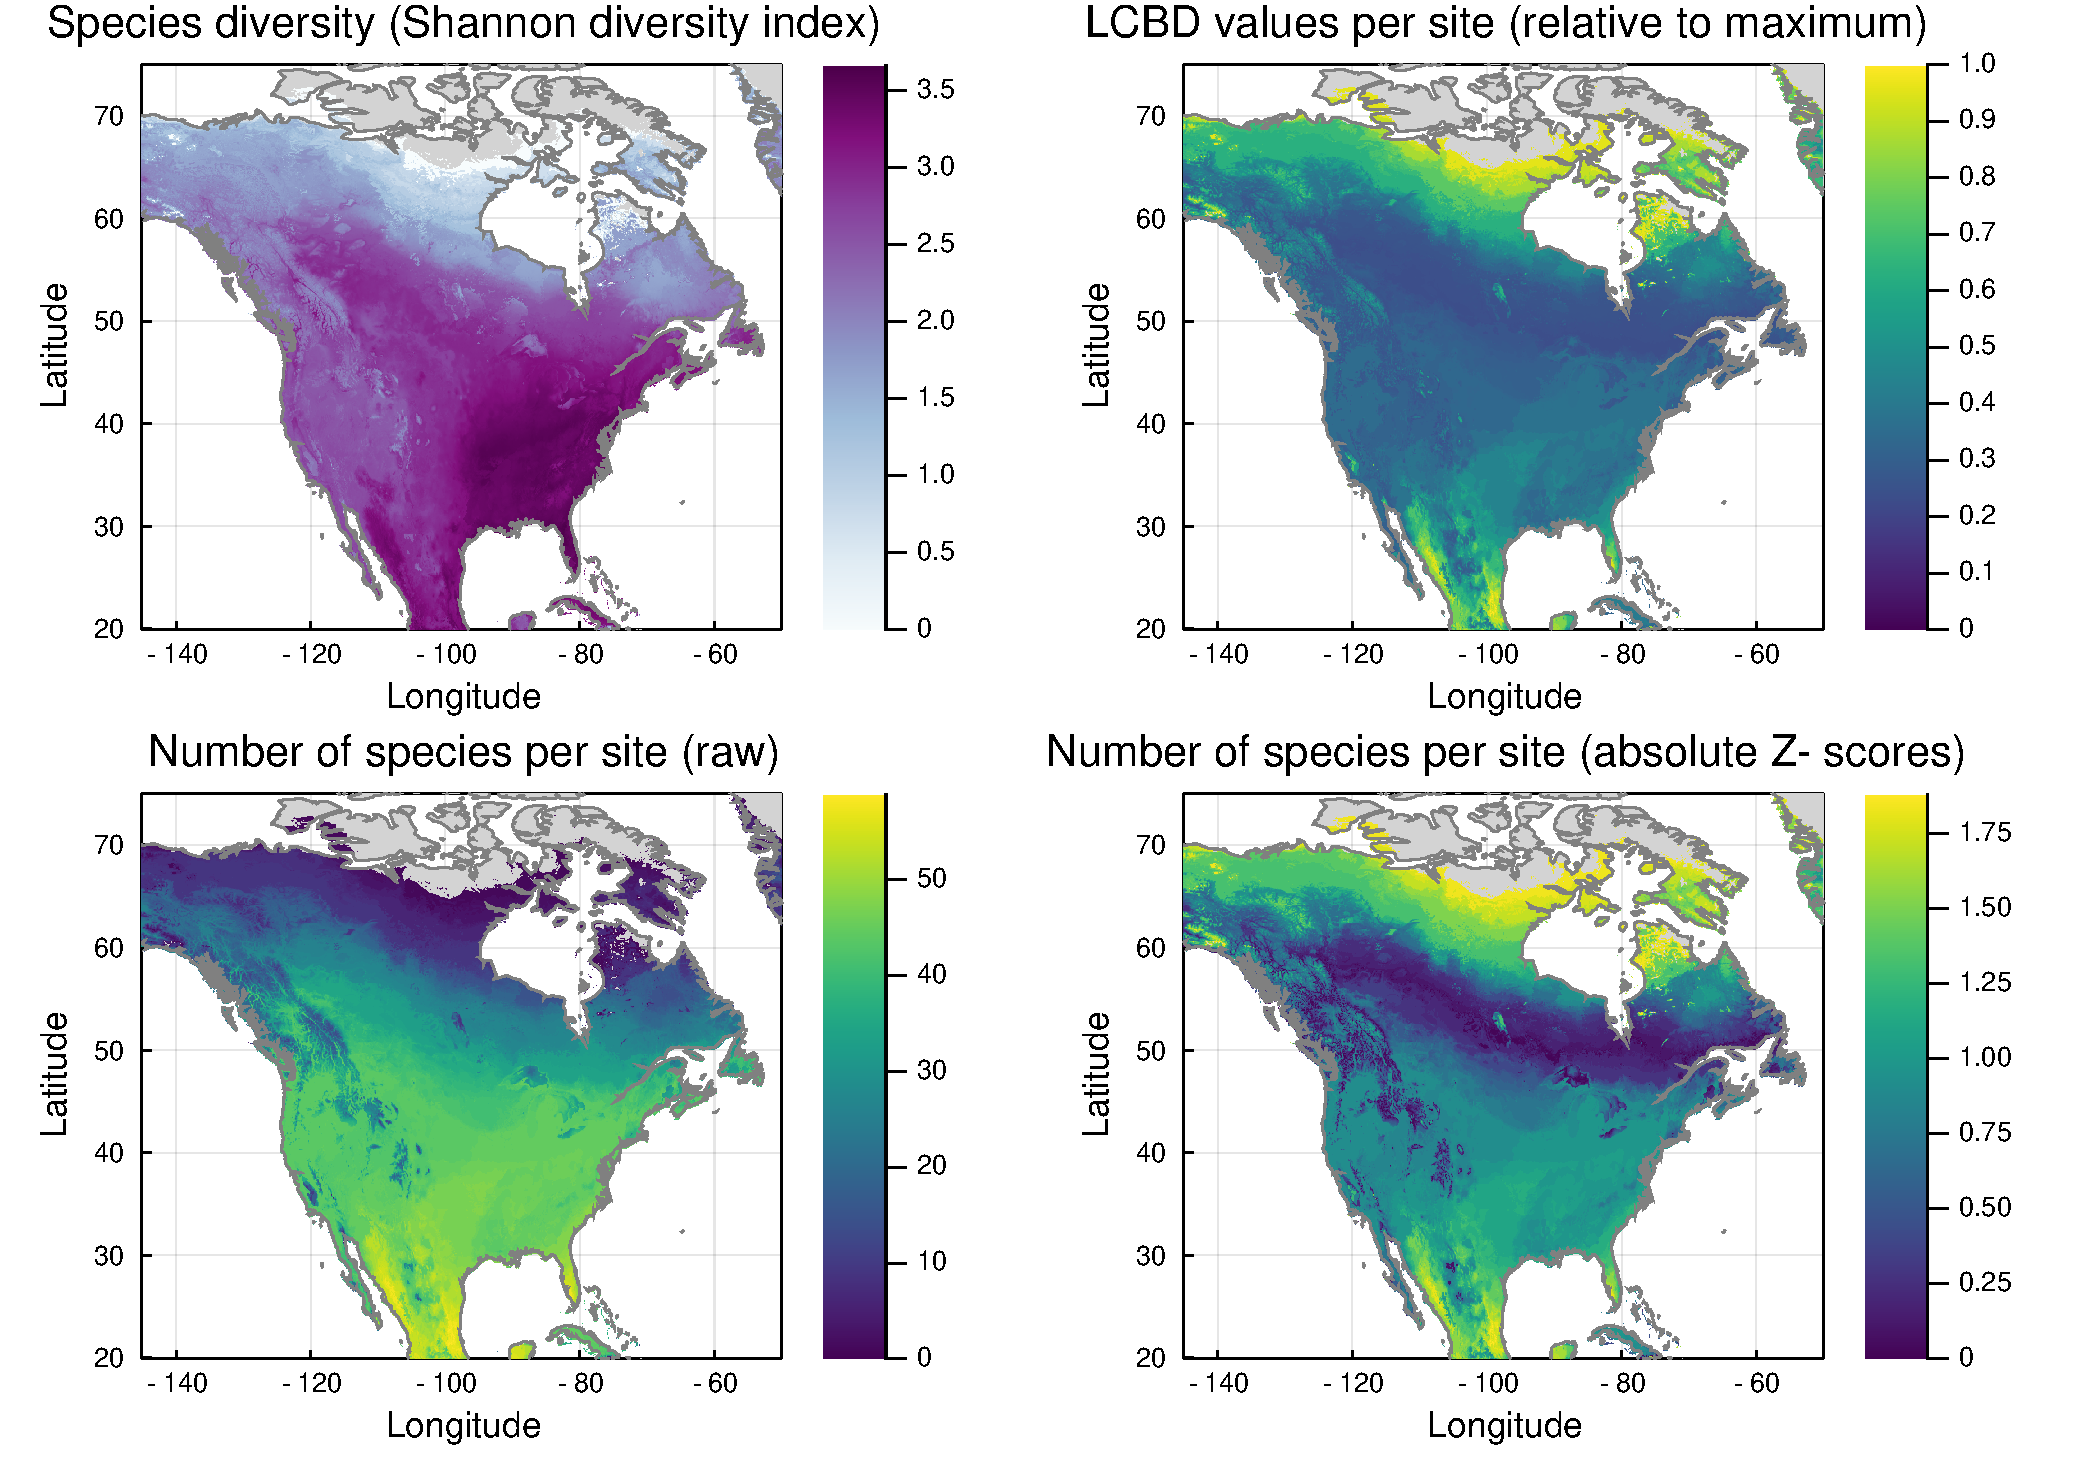
\includegraphics[scale=0.32]{fig/comparison-ebd.pdf}
  \end{figure}
\end{frame}

\begin{frame}
  \frametitle{Résultats - Diversité spécifique}
  \begin{figure}
    \centering
    \includegraphics[scale=0.4]{fig/diversity-ebd.pdf}
  \end{figure}
\end{frame}

\begin{frame}
  \frametitle{Résultats - LCBD}
  \begin{figure}
    \centering
    \includegraphics[scale=0.4]{fig/lcbd-ebd.pdf}
  \end{figure}
\end{frame}

\begin{frame}
  \frametitle{Résultats - Richesse spécifique (nombre d'espèces)}
  \begin{figure}
    \centering
    \includegraphics[scale=0.4]{fig/richness-ebd.pdf}
  \end{figure}
\end{frame}

\begin{frame}
  \frametitle{Résultats - Richesse spécifique (zscores absolus)}
  \begin{figure}
    \centering
    \includegraphics[scale=0.4]{fig/richness-ebd-zscores.pdf}
  \end{figure}
\end{frame}

\begin{frame}
  \frametitle{Résultats - LCBD significatives}
  \begin{figure}
    \centering
    \includegraphics[scale=0.4]{fig/lcbd-ebd-significant.pdf}
  \end{figure}
\end{frame}

\begin{frame}
  \frametitle{Résultats - LCBD sur données osbervées (avant SDM)}
  \begin{figure}
    \centering
    \includegraphics[scale=0.4]{fig/pres-abs-ebd.pdf}
  \end{figure}
\end{frame}

\end{document}
